%%%%%%%%%%%%%%%%%%%%%%%%%%%%%%%%%%%%%%%%%
% Short Sectioned Assignment
% LaTeX Template
% Version 1.0 (5/5/12)
%
% This template has been downloaded from:
% http://www.LaTeXTemplates.com
%
% Original author:
% Frits Wenneker (http://www.howtotex.com)
%
% License:
% CC BY-NC-SA 3.0 (http://creativecommons.org/licenses/by-nc-sa/3.0/)
%
%%%%%%%%%%%%%%%%%%%%%%%%%%%%%%%%%%%%%%%%%

%----------------------------------------------------------------------------------------
%	PACKAGES AND OTHER DOCUMENT CONFIGURATIONS
%----------------------------------------------------------------------------------------

\documentclass[paper=a4, fontsize=11pt]{scrartcl} % A4 paper and 11pt font size
\usepackage[utf8]{inputenc}
\usepackage[MeX]{polski}
\usepackage[T1]{fontenc} % Use 8-bit encoding that has 256 glyphs
\usepackage{fourier} % Use the Adobe Utopia font for the document - comment this line to return to the LaTeX default
 % English language/hyphenation
\usepackage{amsmath,amsfonts,amsthm} % Math packages
\usepackage{graphicx} %images
\usepackage{placeins}%for direct positioning
\usepackage{lipsum} % Used for inserting dummy 'Lorem ipsum' text into the template

\usepackage{wrapfig}
\usepackage{subfig}

\usepackage{sectsty} % Allows customizing section commands
\allsectionsfont{\centering \normalfont\scshape} % Make all sections centered, the default font and small caps

\usepackage{fancyhdr} % Custom headers and footers
\pagestyle{fancyplain} % Makes all pages in the document conform to the custom headers and footers
\fancyhead{} % No page header - if you want one, create it in the same way as the footers below
\fancyfoot[L]{} % Empty left footer
\fancyfoot[C]{} % Empty center footer
\fancyfoot[R]{\thepage} % Page numbering for right footer
\renewcommand{\headrulewidth}{0pt} % Remove header underlines
\renewcommand{\footrulewidth}{0pt} % Remove footer underlines
\setlength{\headheight}{13.6pt} % Customize the height of the header

\numberwithin{equation}{section} % Number equations within sections (i.e. 1.1, 1.2, 2.1, 2.2 instead of 1, 2, 3, 4)
\numberwithin{figure}{section} % Number figures within sections (i.e. 1.1, 1.2, 2.1, 2.2 instead of 1, 2, 3, 4)
\numberwithin{table}{section} % Number tables within sections (i.e. 1.1, 1.2, 2.1, 2.2 instead of 1, 2, 3, 4)

\setlength\parindent{0pt} % Removes all indentation from paragraphs - comment this line for an assignment with lots of text

%----------------------------------------------------------------------------------------
%	TITLE SECTION
%----------------------------------------------------------------------------------------

\newcommand{\horrule}[1]{\rule{\linewidth}{#1}} % Create horizontal rule command with 1 argument of height

\title{	
\normalfont \normalsize 
\textsc{Uniwersytet Wrocławski} \\ [25pt] % Your university, school and/or department name(s)
\horrule{0.5pt} \\[0.4cm] % Thin top horizontal rule
\huge Przybliżanie Okręgu \\
\large Pracownia 3.3 \\ % The assignment title
\horrule{2pt} \\[0.5cm] % Thick bottom horizontal rule
}

\author{Antoni Tomaszewski} % Your name

\date{\normalsize\today} % Today's date or a custom date

\begin{document}

\maketitle % Print the title

%----------------------------------------------------------------------------------------
%	PROBLEM 1
%----------------------------------------------------------------------------------------

\section{Opis problemu}
Tematem zadania jest konstrukcja algorytmu będącego w stanie wyznaczyć przybliżone równanie okręgu. Dowolny punkt na okręgu można wyznaczyć w zależności od kąta $t$, wtedy ma on współrzędne $(cos(t), sin(t))$.  \\
Zadanie możemy więc potraktować jako problem obliczenia funkcji parametrycznej $f(t) \simeq (cos(t), sin(t))$. Zauważmy również, że $cos(t) = sin(t+\frac{\pi}{2})$, zatem wystarczy wyznaczyć przybliżenie $sinusa$ a $cosinusa$ można łatwo z niego obliczyć. W pracy zostaną przedstawione różne podejścia do wykonania tego zadania: za pomocą interpolacji Hermite'a, krzywych Beziera oraz naturalnej funkcji sklejanej.

\medbreak
Implementacja algorytmu została wykonana w języku Julia w pliku "program.jl".
Funkcje pomocnicze zawarte są w pliku "funkcje.jl''.
Wykresy zostały wygenerowane korzystając z biblioteki "Plots".
Do wygodnego używania wielomianów w splajnach użyta została biblioteka "Polynomials''.

\section{Interpolacja Hermite'a}

\subsection{Wprowadzenie}
Interpolacja Hermite'a jest to często używana metoda numeryczna służąca do znalezienia wielomianu przybliżającego mając dane wartości funkcji w $n$ punktach oraz ich $k$ pierwszych pochodnych (dla każdego punktu $k$ może być różne oraz zakładamy że one istnieją). Metoda ta jest bardzo podobna do interpolacji Newtona z tym że u Newtona dla każdego punktu znana jest jedynie jego wartość a u Hermite'a znamy również pewną ilość pochodnych w tym punkcie. Interpolacja Hermite'a jest więc rozszerzeniem interpolacji Newtona.\\ 
Łatwo zauważyć że gdy nie znamy wartości w wielu punktach, ale za to znamy wiele wartości kolejncyh pochodnych w tych punktach Hermite będzie bardzo wygodną i znacznie bardziej dokładną metodą niż Newton. Z tej obserwacji korzystać będzie pierwsza z metod służących konstrukcji okręgu.

\subsection{Zastosowanie w konstrukcji okręgu}
Konstrukcja fragmentu łuku okręgu na przedziale $[-\alpha, \alpha]$ została opisana w artykule \cite{hermite}. Punktami w których będziemy interpolować funkcję $cosinus$ (oraz $sinus$) będą krańce przedziału, czyli $\alpha$ i $-\alpha$, chcąc osiągnąć stopień wielomianu $2n+1$ będziemy potrzebować wartości $n$ pierwszych pochodnych w tych punktach. \\
Główna idea stojąca za algorytmem w nim przestawionym polega na tym, aby dokonać rozwinięcia w szereg Taylora w dwóch punktach : $\alpha$ i $-\alpha$.
\begin{gather}
f(x) = f(\alpha) + f'(\alpha)\frac{x-\alpha}{1!} + f''(\alpha)\frac{(x-\alpha)^{2}}{2!} + ... \\
w_{n}(x) = f(\alpha) + f'(\alpha)\frac{x-\alpha}{1!} + f''(\alpha)\frac{(x-\alpha)^{2}}{2!} + ... + f^{(n)}(\alpha)\frac{(x-\alpha)^{n}}{n!} \\
f(x) = f(-\alpha) + f'(-\alpha)\frac{x+\alpha}{1!} + f''(-\alpha)\frac{(x+\alpha)^{2}}{2!} + ... \\
v_{n}(x) = f(-\alpha) + f'(-\alpha)\frac{x+\alpha}{1!} + f''(-\alpha)\frac{(x+\alpha)^{2}}{2!} + ... + f^{(n)}(-\alpha)\frac{(x+\alpha)^{n}}{n!}
\end{gather}
Następnie obliczyć wartości w punktach krańcowych tych funkcji oraz wartości pierwszych $n$ pochodnych tych funkcji. \\
Chcemy więc, by zachodziły nastęujące równości:
\begin{gather*}
w_{n}(\alpha) = f(\alpha) \\
w_{n}'(\alpha) = f'(\alpha) \\
...\\
w_{n}^{(n)}(\alpha) = f^{(n)}(\alpha)
\end{gather*}
oraz
\begin{gather*}
v_{n}(\alpha) = f(\alpha) \\
v_{n}'(\alpha) = f'(\alpha) \\
...\\
v_{n}^{(n)}(\alpha) = f^{(n)}(\alpha)
\end{gather*}
Po przejściu przez stertę obliczeń otrzymujemy następujące wzory \\
$$  C_{2n+1}(\alpha, t) = (cos\alpha + 2\sum_{k=1}^{n} x_{k}(t^{2} - \alpha^{2})^{k},  \frac{sin\alpha}{\alpha}t + 2t\sum_{k=1}^{n} y_{k}(t^{2} - \alpha^{2})^{k}) $$ gdzie \\
$$x_{k} = \frac{1}{k!}\sum_{i=0}^{k-1} \frac{(k+i-1)!}{i!(k-i-1)!} \frac{cos(\frac{k+i}{2}\pi + \alpha)}{(2\alpha)^{k+i+1}} $$ \\
oraz $$ y_{k} = -2\alpha(k+1)x_{k+1} $$ \medbreak
Zauważmy, że mając fragment łuku postaci $[(x_{1},y_{1}), (x_{2},y_{2}), ..., (x_{k}, y_{k})]$ możemy odbić go względem prostej przechodzącej przez punkty
$(x_{1},y_{1})$ oraz $(0,0)$ i otrzymać tym sposobem dwukrotnie dłuższy łuk. Z tej obserwacji można skorzystać  i uzyskać zadowalające wyniki dla niewielkich stopni wielomianów.
\subsection{Wyniki}
\begin{figure}[h!]
\centering
 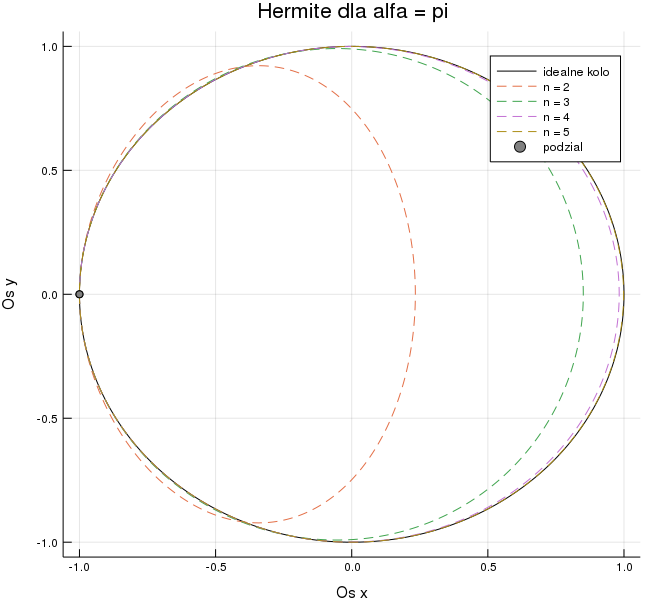
\includegraphics[width=0.8\linewidth]{hermite.png}
  \caption{Okrąg za pomocą hermite'a przy przedziale interpolacji $[\alpha, -\alpha]$, 0 odbić}
  \label{hermite}
\end{figure}

\begin{figure}[h!]
\centering
 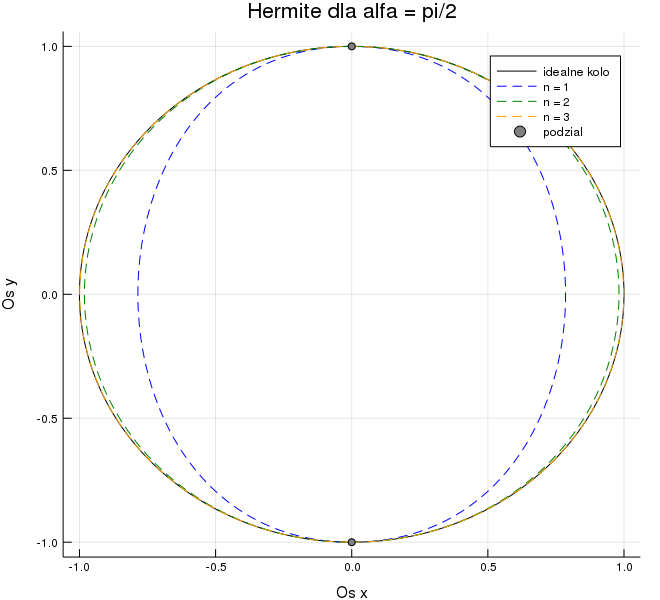
\includegraphics[width=0.8\linewidth]{hermitedwa.png}
  \caption{Okrąg za pomocą hermite'a przy przedziale interpolacji $[\frac{\alpha}{2}, \frac{-\alpha}{2}]$ , 1 odbicie}
  \label{hermitedwa}

 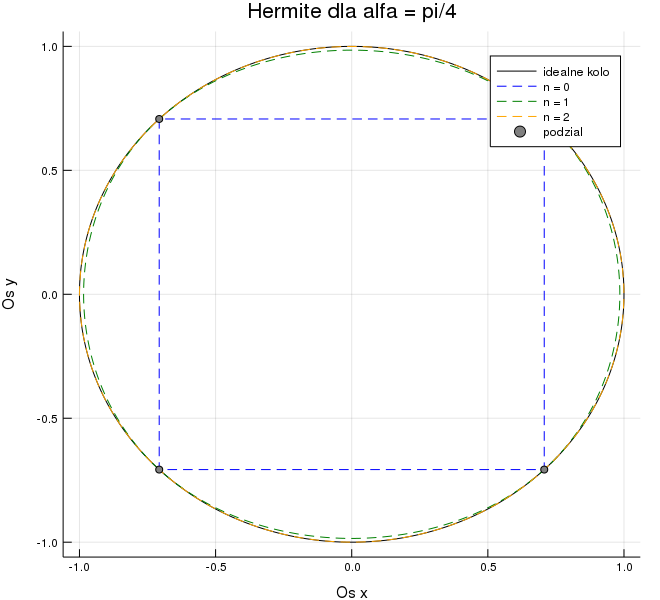
\includegraphics[width=0.8\linewidth]{hermitetrzy.png}
  \caption{Okrąg za pomocą hermite'a przy przedziale interpolacji $[\frac{\alpha}{4}, \frac{-\alpha}{4}]$, 2 odbicia}
  \label{hermitetrzy}
\end{figure}

\FloatBarrier
Zauważmy, że na ''oko'' porównywalne wydają się wyniki kolejnych rysunków dla $n = 4$, $n=2$, $n=1$. 













\section{Krzywe Beziera}
\subsection{Wprowadzenie}
Krzywe Beziera to częsta i dosyć prosta technika wykorzystywana w grafice komputerowej. Polega na wybraniu $n+1$ punktów $(P_{0}, ... , P_{n})$ zwanymi punktami kontrolnymi. Funkcja wynikowa będzie przechodzić przez pierwszy i ostatni punkt oraz nie przechodzić przez żaden pozostały. Funkcja takej krzywej dla dowolnej liczby punktów kontrolnych wyraża się wzorem 
\begin{align}
B(t) = (1-t)^{n}P_{0} + {{n}\choose{1}}(1-t)^{n-1}tP_{1} + ... + {{n}\choose{n-1}}(1-t)t^{n-1}P_{n-1} + t^{n}P_{n}
\end{align}
Gdzie wyrażenie przy $k-tym$ punkcie ($P_{k}$) to $k-ty$ wielomian Bernsteina stopnia $n$.

\subsection{Zastosowanie w konstrukcji okręgu}
Do wyznaczenia okręgu użyjemy wielomianu stopnia 3. W następujących punktach kontrolnych: $[(0,1), (c,1), (1,c), (0,1)]$, gdzie $c = \frac{4}{3}(\sqrt{2} - 1)$. Wartość $c$ można wyliczyć z wielomianu $B(t)$ dla punktu $(0.5, 0.5)$, który leży na tej krzywej.


\begin{figure}[h!]
\centering
 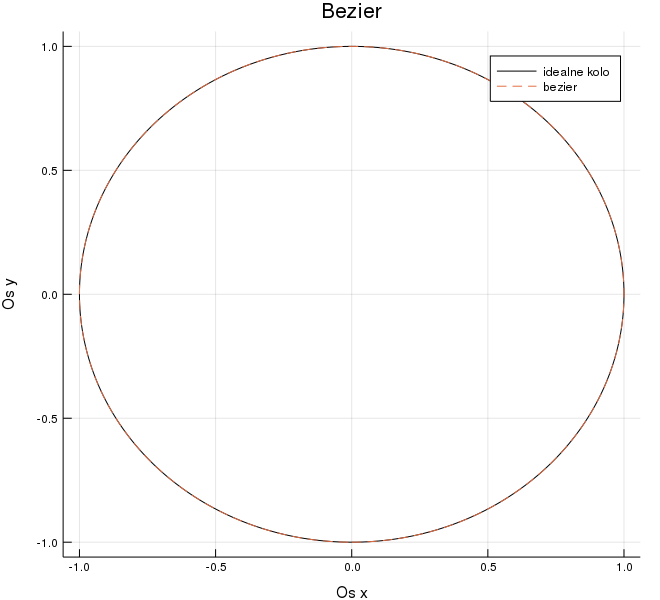
\includegraphics[width=0.68\linewidth]{bezier.png}
  \caption{Wykres okręgu uzyskanego za pomocą krzywych Beziera}
  \label{bezier}
\end{figure}
\FloatBarrier


\section{Naturalna funkcja sklejana}
\subsection{Wprowadzenie}
Splajn jest często wykorzystywaną i uniwersalną techniką interpolacji. Jest ''odporny'' na efekt Rungego oraz działa dla dowolnego wyboru punktów (zarówno równoodległych jak i nie). W miarę zwiększania ilości danych metoda ta staje się bardziej dokładna. Technika polega na stworzeniu, dla każdej pary sąsiednich punktów, wielomianu stopnia co najwyżej trzeciego,w taki sposób aby wykres był gładki oraz ciągły.
\medbreak
Mając $n+1$ punktów $(x_{1},y_{1}), (x_{2},y_{2}) ... (x_{n+1}, y_{n+1})$ chcemy na każdym z przedziałów $[x_{k}, x_{k+1}]$ skonstruować wielomian $3$ st. \\
Niech
\begin{gather}
 s_{k}(x) = A_{k} + B_{k}(x - x_{k}) + C_{k}(x - x_{k})^{2} + D_{k}(x - x_{k})^{3} \\
 s_{k}'(x) = B_{k} + 2C_{k}(x - x_{k}) + 3D_{k}(x - x_{k})^{2} \\
 s_{k}''(x) = 2C_{k}+ 6D_{k}(x - x_{k}) \\
\end{gather}
Chcemy więc mieć $n$ funkcji i dla każdej z nich $4$ warunki, co daje w sumie $4n$ warunków. \\
$n+1$ punktów daje nam $2n$ warunków ($n-1$ podwójnych oraz dwa pojedyncze (brzegowe))
Żądamy również, aby pierwsze oraz drugie pochodne na krańcach przedziałów były sobie równe (kolejne $2(n-1)$ warunków).
\begin{align}
s_{k+1}'(x_{k+1}) = s_{k}'(x_{k+1}) \\
s_{k+1}''(x_{k+1}) = s_{k}''(x_{k+1})
\end{align}
Brakuje nam jeszcze dwóch warunków, które zapewniamy sobie ustawiając wartości drugich pochodnych w punktach brzegowych na $0$.
\begin{align}
s_{1}''(x_{1}) = s_{n}''(x_{n+1}) = 0
\end{align}
\subsection{Zastosowanie w konstrukcji okręgu}
Użycie splajnów do tego zadania wydaje się sensownym pomysłem, ponieważ wraz z zwiększaniem ilości punktów wykres staje się coraz bardziej dokładny, czego nie gwarantują nam interpolacja Netwona ani interpolacja Lagrange'a. 
\begin{figure}[h!]
\centering
 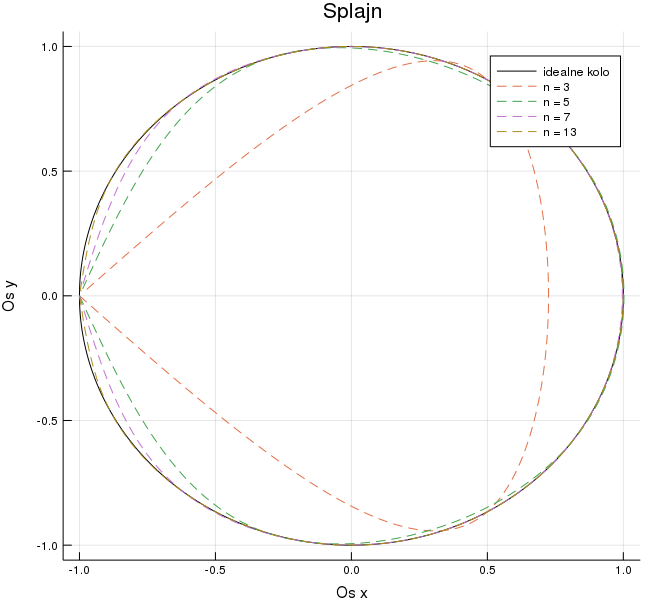
\includegraphics[width=0.8\linewidth]{splajn.png}
  \caption{Wykres Splajna dla punktów równoodległych, gdzie n = liczba węzłów interpolacyjnych}
  \label{przedzialy}
\end{figure}
\FloatBarrier

\section{Helisa}
W artykule \cite{hermite} jest opisane jak z wykresu koła uzyskać helisę. Możemy ją obliczyć korzystając z każdej z trzech wyżej opisanych metod, a jej dokładność będzie zależeć jedynie od dokładności wcześniej obliczonego wykresu okręgu, dlatego można przy porównaniu tych metod ograniczyć się do zestawienia jedynie dokładności okręgów. \\
Helisę opisuje wzór: $H(\alpha, t) = (\cos t, \sin t, t)$, $t \in [-\pi, \pi]$
\begin{figure}[h!]
 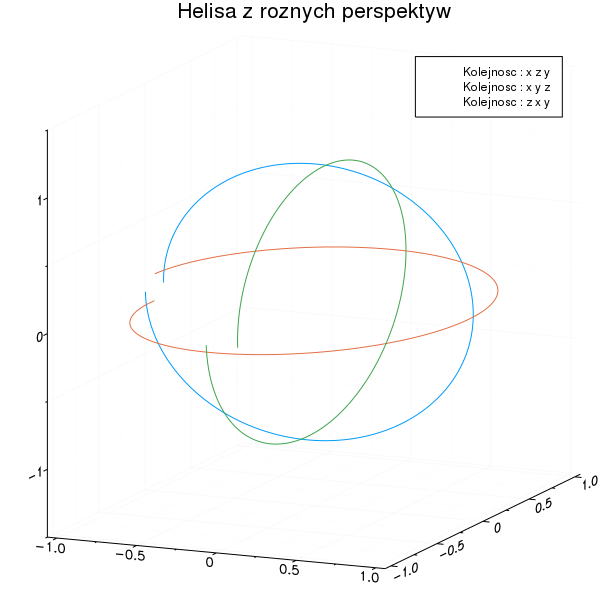
\includegraphics[width=0.8\linewidth]{hermitehelisa.png}
  \caption{Wykres Helisy za pomocą Hermite'a, różne widoki}
  \label{helisa}
\end{figure}
\FloatBarrier

\section{Porównanie}
Poniżej przedstawione są błędy, z których wynikają następujące własności: 
\medbreak
Dla wielomianów stopnia 3 najmniejsze maksimum z błędów ma Bezier, równe $0.007$. Wykorzystuje on $2$ wielomiany sześcienne, więc używa $8$ współczynników. \\
Maksimum błędów Hermite'a dla $\alpha = \frac{\pi}{4}$, $n = 1$ (czyli 2  wielomianów st. $3$) wynosi $0.015$, również 8 współczynników \\
Natomiast splajn osiąga porównywalne maksimum błędu co Bezier dla 17 funkcji sklejanych ($4 * 17 = 68$ współczynników). 
\medbreak
Analizując Hermite'a i splajn, zauważymy że maksimum najgorszego z Hermite'ów czyli  $\alpha = \pi$, $n = 4$ jest porównywalne z splajnem dla $n = 11$.\\ $20$ współczynników u Hermite'a przeciw $44$ w splajnach.
\medbreak
Patrząc wyłącznie na wyniki w splajnach widzimy, że chociaż na większości przedziału błąd jest niewielki, to jednak na krańcach zawsze osiąga całkiem duże wartości.


\begin{figure}
\centering
{\label{hermite}
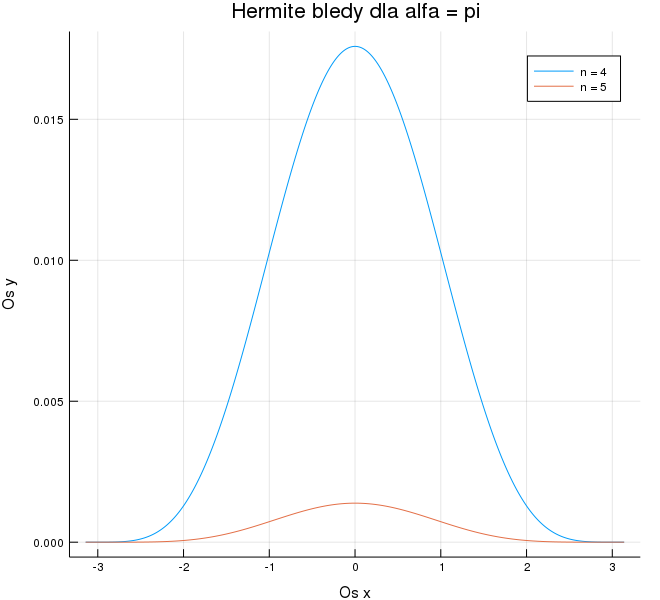
\includegraphics[width=0.45\textwidth]{hermitebledy}}
\quad
{\label{hermite}
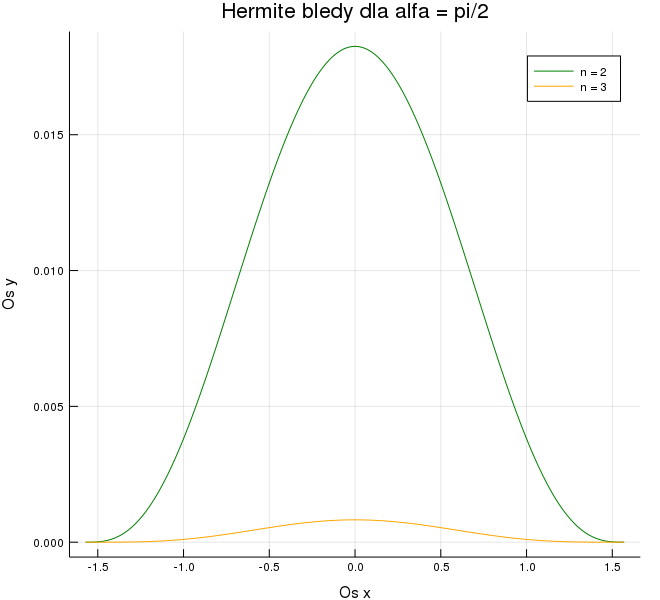
\includegraphics[width=0.45\textwidth]{hermitedwabledy}}
\end{figure}
\begin{figure}
\centering
{\label{hermite}
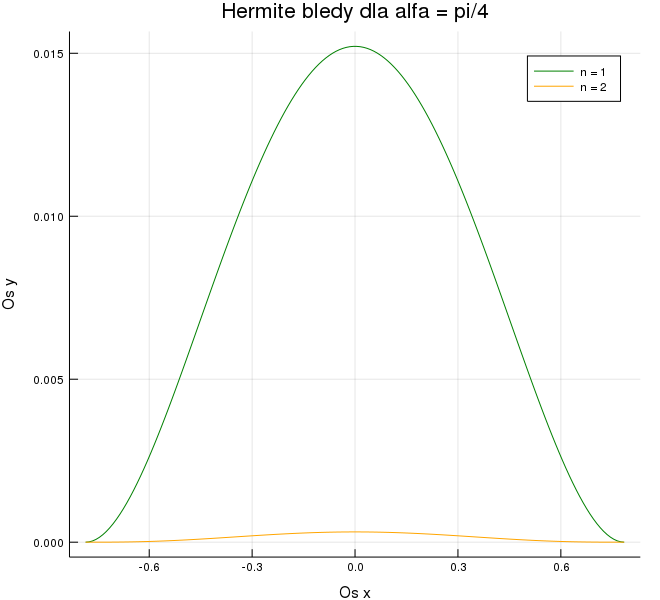
\includegraphics[width=0.45\textwidth]{hermitetrzybledy}}
\quad
{\label{hermite}
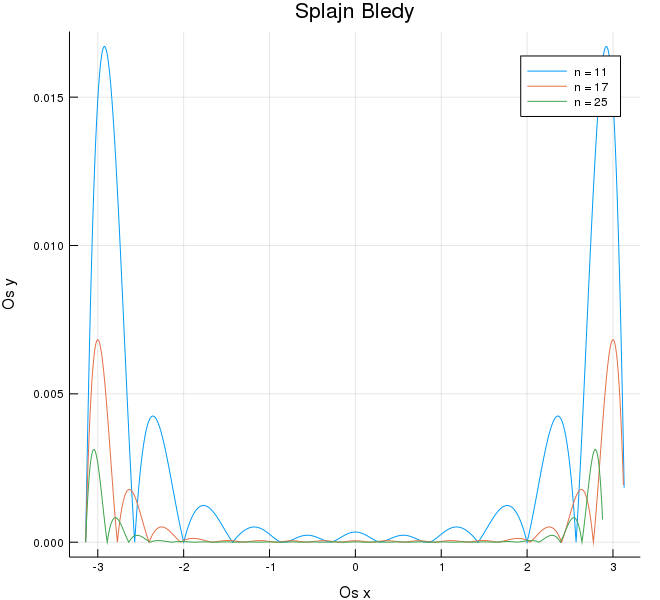
\includegraphics[width=0.45\textwidth]{splajnbledy}}
\end{figure}
\begin{figure}
\centering
{\label{hermite}
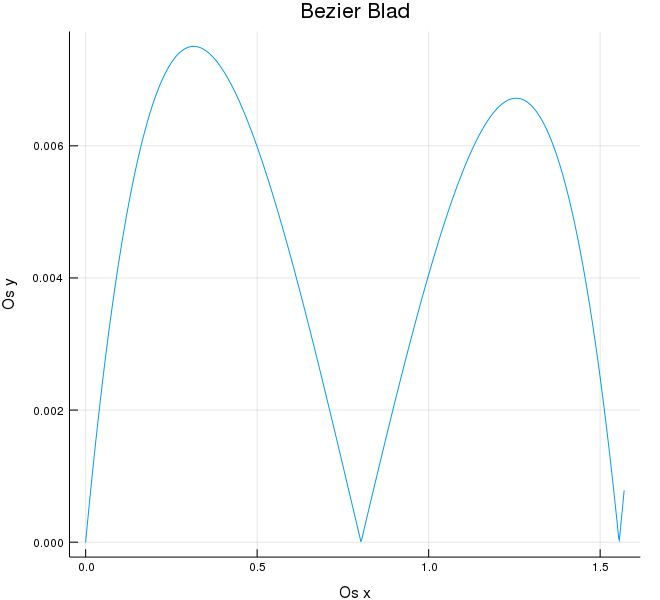
\includegraphics[width=0.45\textwidth]{bezierblad}}
\end{figure}



\FloatBarrier

\section{Wnioski}
Wybranie odpowiedniej metody powinno zależeć od problemu, jaki mamy rozwiązać. Krzywe Beziera oraz naturalne funkcje sklejane są metodami bardziej ogólnymi niż algorytm opisany w \cite{hermite}, nie powinno stanowić więc zaskoczenia, że radzą sobie one z przybliżeniem okręgu gorzej niż sposób do tego jedynie dedykowany.  Jeśli chcielibyśmy użyć jak najmniej danych należałoby skorzystać z krzywych Beziera. Jednak w sytuacji, gdy priorytetem jest precyzja istnieje lepsze rozwiązanie. Jest nim metoda zawarta w artykule \cite{hermite}. Używa mniej danych, a błąd ma istotnie mniejszy oraz bardziej stabilny niż splajn oraz Bezier.
\begin{thebibliography}{9}

\bibitem{hermite}
  Lizheng Lu
  \textit{On polynomial approximation of circular arcs and helices}, \\
  Department of Mathematics, \\
  Zhejiang Gongshang University, \\
  2011
    
\bibitem{taylor}
 J.L.López,
 N.M.Temme,
 \textit{Two-point Taylor expansions of analytic functions},\\
 Studies in Applied Mathematics\\
 2002 \\
 str. 297-311
\end{thebibliography}

\end{document}
